\begin{center}
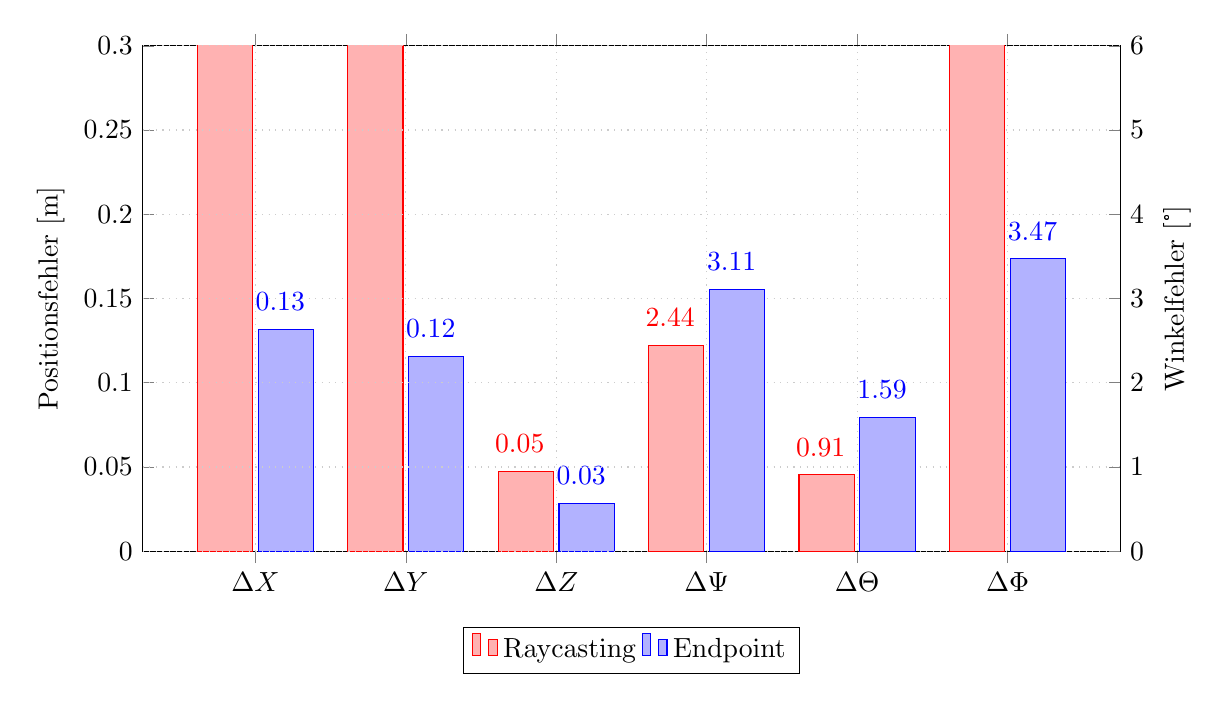
\begin{tikzpicture}
\begin{axis}[
	ybar,
	ymax=0.3,
	ymin=0,
	bar width=20pt,
	scaled y ticks = false,
	y tick label style={/pgf/number format/fixed},
%	enlarge y limits={0.4,upper},
	enlarge x limits=0.15,
	legend style={at={(0.5,-0.15)},
	anchor=north,legend columns=-1},
	ylabel={Positionsfehler \lbrack m\rbrack},
%	symbolic x coords={\Delta,y,z},
	xtick={1,2,3,4,5,6},
	xticklabels={$\Delta X$, $\Delta Y$, $\Delta Z$, $\Delta \Psi$, $\Delta \Theta$, $\Delta \Phi$},
%	xtick=data,
	every node near coord/.style={/pgf/number format/fixed, anchor=west},
	nodes near coords,
	nodes near coords align={vertical},
	width=14cm,
	height=8cm,
	grid=major,
    	grid style={dotted,lightgray!80!white},
    	scaled y ticks = false,
]
\addplot[
	every node near coord/.append style={xshift=-0.9cm},
	nodes near coords=\raisebox{0.7cm}{\pgfmathprintnumber\pgfplotspointmeta},
	color=red,
	fill=red!30!white,
	bar shift=-11pt,
] coordinates {(1,0.3105647208) (2,0.3388888731) (3,0.0473358078)};
\addplot[
	every node near coord/.append style={xshift=-0.12cm},
	nodes near coords=\raisebox{0.7cm}{\pgfmathprintnumber\pgfplotspointmeta},
	color=blue,
	fill=blue!30!white,
	bar shift=11pt,	
] coordinates {(1,0.1315834135) (2,0.1156007492) (3,0.0283533047)};
\addplot[fill opacity=0.0,draw=none,] coordinates {(4,0) (5,0) (6,0)};	%dummy
\legend{Raycasting,Endpoint}
\end{axis}

\begin{axis}[
%	scale only axis,
	ybar,
	ymax=6,
	ymin=0,
	bar width=20pt,
%	enlarge y limits={0.4,upper},
	enlarge x limits=0.15,
	legend style={at={(0.5,-0.15)},
	anchor=north,legend columns=-1},
	axis y line*=right,
	axis x line=none,
	ylabel={Winkelfehler \lbrack °\rbrack},
%	symbolic x coords={\Delta,y,z},
	xtick={1,2,3,4,5,6},
	xticklabels={$\Delta X$, $\Delta Y$, $\Delta Z$, $\Delta \Psi$, $\Delta \Theta$, $\Delta \Phi$},
%	xtick=data,
%	bar shift=0pt,
	every node near coord/.style={/pgf/number format/fixed, anchor=west},
	nodes near coords,
	nodes near coords align={vertical},
	width=14cm,
	height=8cm,
	grid=major,
    	grid style={dotted,lightgray!80!white},
    	scaled y ticks = false,
]
\addplot[fill opacity=0.0,draw=none,] coordinates {(1,0) (2,0) (3,0)};	%dummy
\addplot[
	every node near coord/.append style={xshift=-0.9cm},
	nodes near coords=\raisebox{0.7cm}{\pgfmathprintnumber\pgfplotspointmeta},
	color=Red,
	fill=Red!30!white,
	bar shift=-11pt,	
] coordinates {(4,2.4445637073) (5,0.9069805767) (6,8.4545773848)};
\addplot[
	every node near coord/.append style={xshift=-0.12cm},
	nodes near coords=\raisebox{0.7cm}{\pgfmathprintnumber\pgfplotspointmeta},
	color=Blue,
	fill=Blue!30!white,
	bar shift=11pt,	
] coordinates {(4,3.1097896867) (5,1.5883227312) (6,3.4716845667)};
\end{axis}
\label{fig.glob_loc}
\end{tikzpicture}
\end{center}

%\begin{center}
%\begin{tikzpicture}[trim axis left, trim axis right]
%\begin{axis}[
%	ybar,
%	ymax=0.4,
%	ymin=0,
%	bar width=30pt,
%	enlarge x limits=0.4,
%	legend style={at={(0.5,-0.15)},
%	anchor=north,legend columns=-1},
%	ylabel={Positionsfehler \lbrack m\rbrack},
%%	symbolic x coords={\Delta,y,z},
%	xticklabels={$\Delta X$, $\Delta Y$, $\Delta Z$},
%	xtick=data,
%	every node near coord/.style={/pgf/number format/fixed, anchor=west},
%	nodes near coords,
%	nodes near coords align={vertical},
%	width=14cm,
%	height=8cm,
%	grid=major,
%    	grid style={dotted,lightgray!80!white},
%    	scaled y ticks = false,
%]
%\addplot[
%	every node near coord/.append style={xshift=-1.1cm},
%	nodes near coords=\raisebox{0.7cm}{\pgfmathprintnumber\pgfplotspointmeta},
%	color=red,
%	fill=red!30!white
%] coordinates {(-1,0.3105647208) (0,0.3388888731) (1,0.0473358078)};
%\addplot[
%	every node near coord/.append style={xshift=0.0cm},
%	nodes near coords=\raisebox{0.7cm}{\pgfmathprintnumber\pgfplotspointmeta},
%	color=blue,
%	fill=blue!30!white
%] coordinates {(-1,0.1315834135) (0,0.1248760865) (1,0.0209899568)};
%\legend{Raycasting,Endpoint}
%\end{axis}
%\label{fig.error_glob_trans}
%\end{tikzpicture}
%\end{center}
%
%\red[Winkelfehler Vergleich:\\]
%
%\begin{center}
%\begin{tikzpicture}[trim axis left, trim axis right]
%\begin{axis}[
%	ybar,
%	ymax=10,
%	ymin=0,
%	bar width=30pt,
%%	enlarge y limits={0.4,upper},
%	enlarge x limits=0.4,
%	legend style={at={(0.5,-0.15)},
%	anchor=north,legend columns=-1},
%	ylabel={Winkelfehler \lbrack °\rbrack},
%%	symbolic x coords={\Delta,y,z},
%	xticklabels={$\Delta \Psi$, $\Delta \Theta$, $\Delta \Phi$},
%	xtick=data,
%	every node near coord/.style={/pgf/number format/fixed, anchor=west},
%	nodes near coords,
%	nodes near coords align={vertical},
%	width=14cm,
%	height=8cm,
%	grid=major,
%    	grid style={dotted,lightgray!80!white},
%    	scaled y ticks = false,
%]
%\addplot[
%	every node near coord/.append style={xshift=-1.1cm},
%	nodes near coords=\raisebox{0.7cm}{\pgfmathprintnumber\pgfplotspointmeta},
%	color=red,
%	fill=red!30!white
%] coordinates {(-1,2.4445637073) (0,0.9069805767) (1,8.4545773848)};
%\addplot[
%	every node near coord/.append style={xshift=0.0cm},
%	nodes near coords=\raisebox{0.7cm}{\pgfmathprintnumber\pgfplotspointmeta},
%	color=blue,
%	fill=blue!30!white
%] coordinates {(-1,3.1694824628) (0,1.6633422885) (1,4.2398218425)};
%\legend{Raycasting,Endpoint}
%\end{axis}
%\label{fig.error_glob_rot}
%\end{tikzpicture}
%\end{center}


%\begin{figure}[!ht]
%	\begin{center}
%	\subfigure[1. Formparameter (Fokus-Modell)]{
%		\begin{tikzpicture}[scale=0.6, baseline]
%            \begin{axis}[ybar]
%                \addplot+ coordinates {
%                    (1,2)
%                };
%            \end{axis}
%        \end{tikzpicture}
%	}
%	\hspace{2mm}
%	\subfigure[1. Formparameter (Post-Fokus-Modell)]{
%		\begin{tikzpicture}[scale=0.6, baseline]
%            \begin{axis}[ybar]
%                \addplot+ coordinates {
%                    (1,2)
%                };
%            \end{axis}
%        \end{tikzpicture}
%	}\\
%	\caption{Variation der ersten beiden Formparameter um $\pm 3 \sqrt{\lambda_i}$}
%	\label{fig.reference_building_shape_visualization}
%	\end{center}
%	\vspace*{-8mm}
%\end{figure}